% Chapter 2

% variables
\newcommand{\pdirtwo}{chapters/chapter2/plots}

\chapter{The NA64 experiment} % Main chapter title

\label{chapter2} % For referencing the chapter elsewhere, use \ref{Chapter2} 

% ----------------------------------------------------------------------------------------

The second step of any physics experiment, after a clear goal is set, is the design of the setup to perform the test. As we decided to perform an experiment to probe the $\umodel$, the first thing we need to realize is how to produce such type of dark matter in colliders. A the new symmetry theorized is mixed with the well studied symmetry $U(1)$ of the standard model, the channels that allow the production of this new boson $\DM$ are similar to the one that can be used for $\gamma$. The channels that contributes in first order are the following:

\begin{itemize}
\item \textit{Dark Bremsstrahlung}: The reaction $\darkbrem$ where $\DM$ is emitted after a virtual photon is exchanged with a target nucleus.
\item \textit{Dark Compton}: The reaction $\darkcompton$, where $\DM$ is produced as consequence of the interaction of a photon and an electron.
\item \textit{Dark Resonance}: The reaction $\darkresonance$ where two leptons annihilated and produce a $\DM$ as a consequence of a resonance.
\end{itemize}

The Feynman diagrams of all processes mentioned above is depicted in Fig.\ref{fig:dm-production-mechanism}.

% INSER HERE A PICTURE WITH ALL FEYNMAN DIAGRAM OF THE CORRESPONDING CHANNELS
\begin{figure}
  \centering
  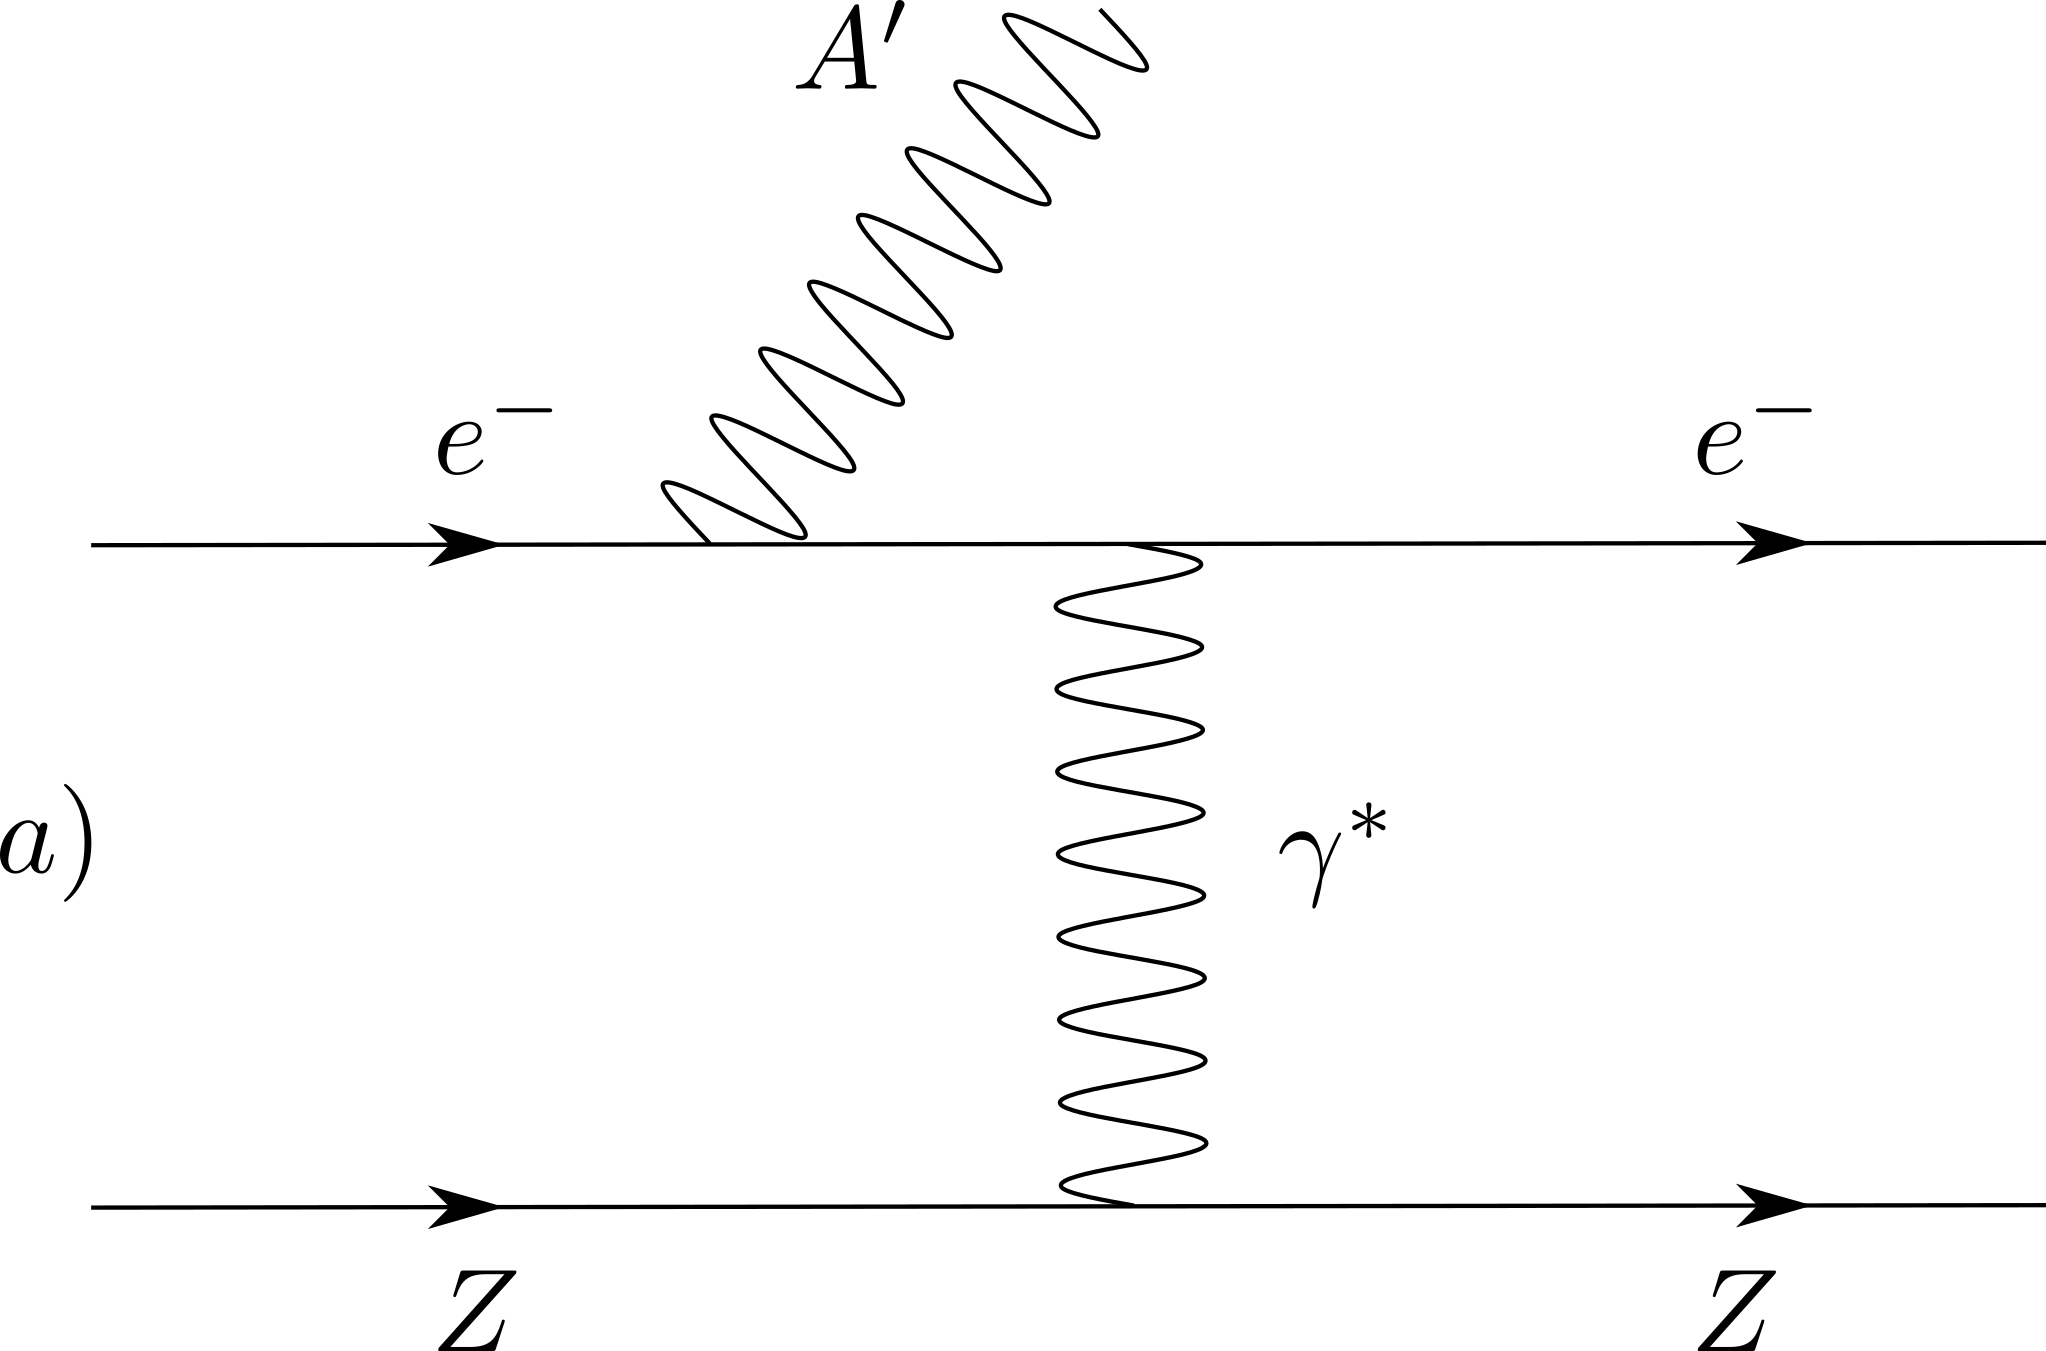
\includegraphics[width=.45\textwidth]{\pdirtwo/DarkBremstrahlung.png}
  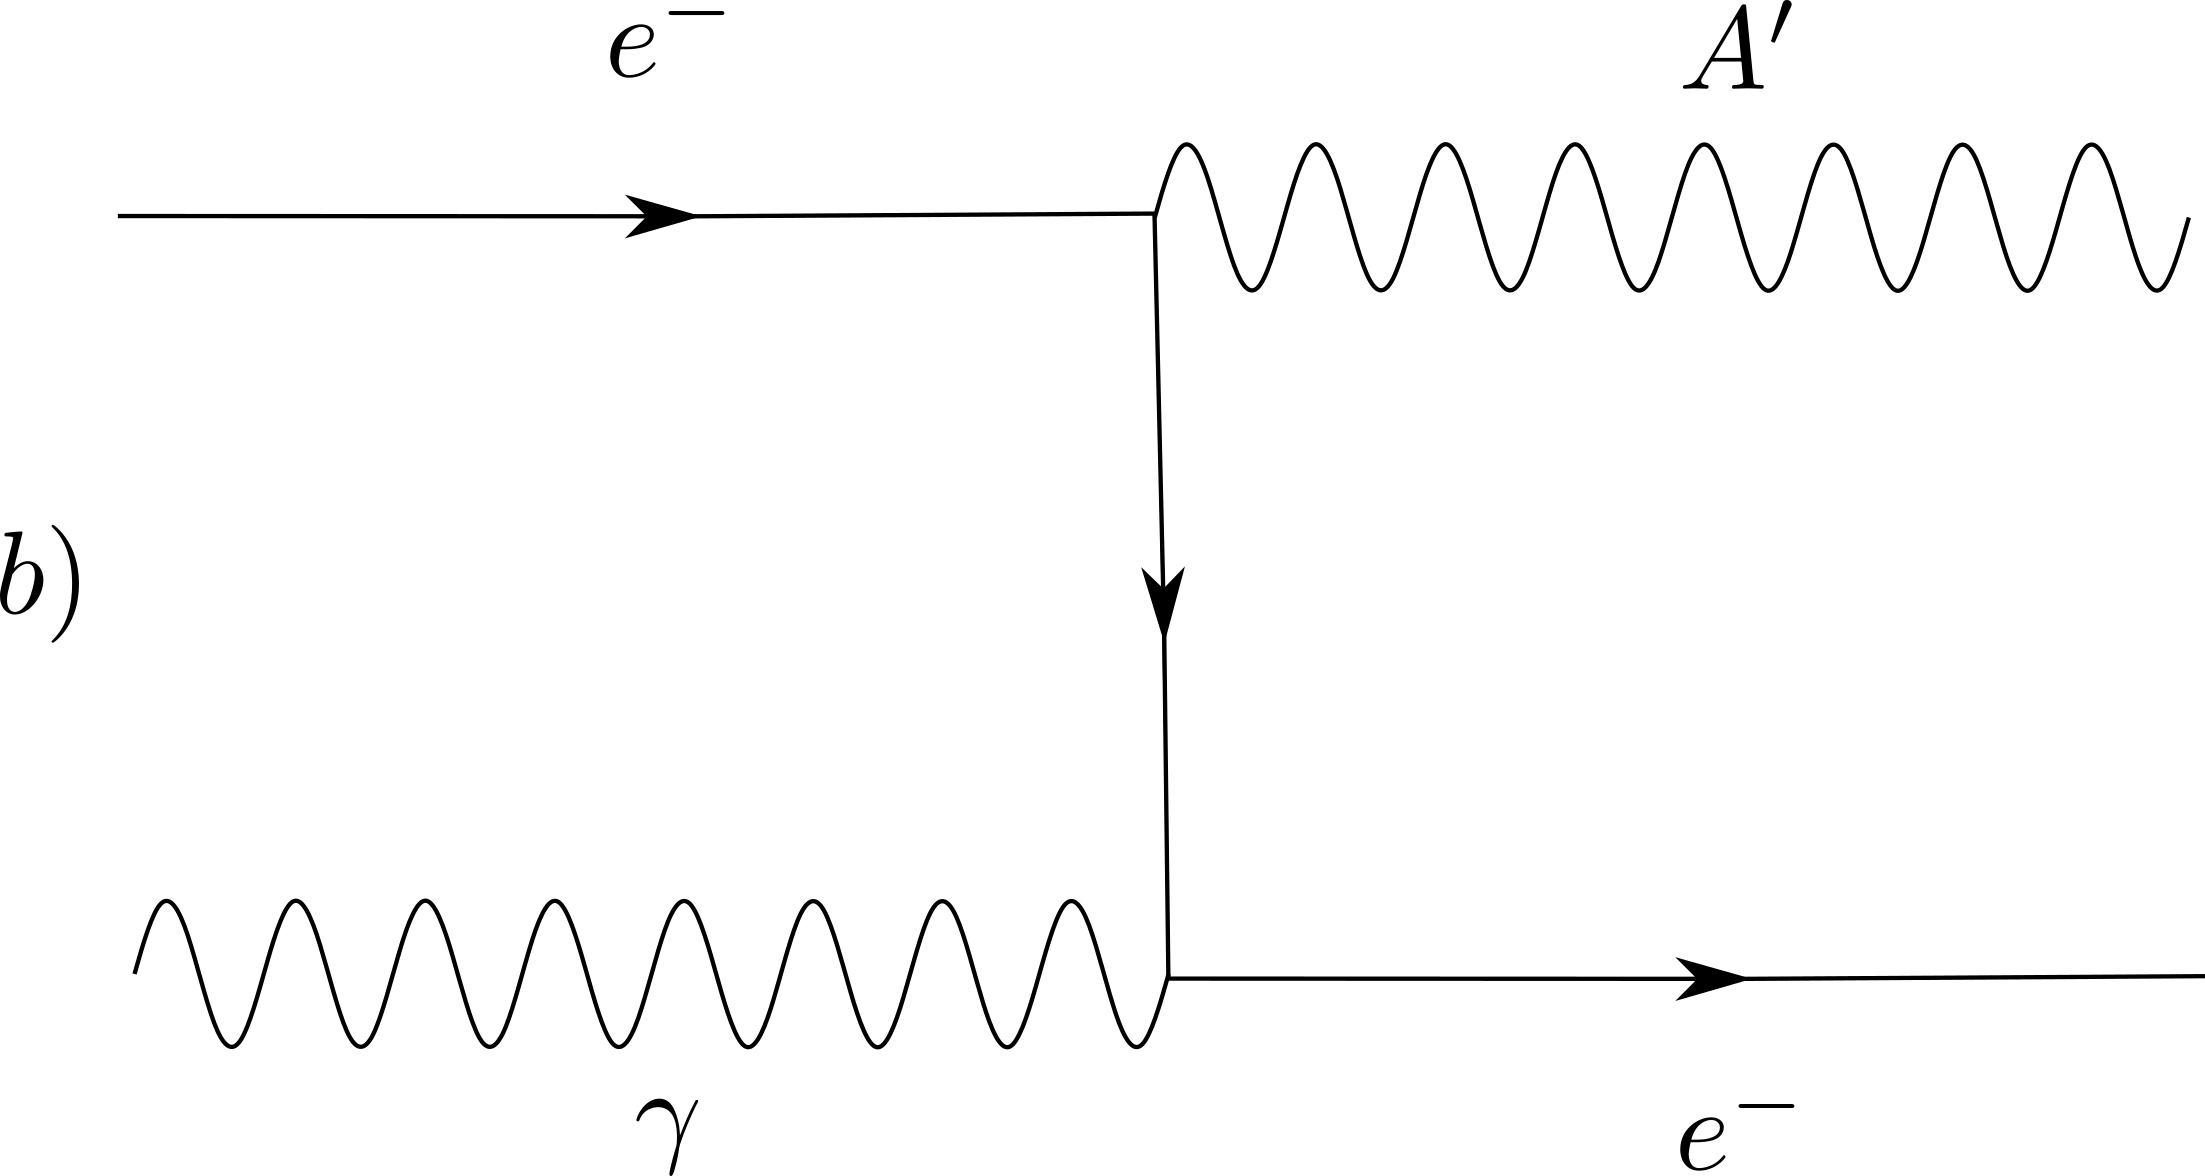
\includegraphics[width=.45\textwidth]{\pdirtwo/DarkCompton.png}
  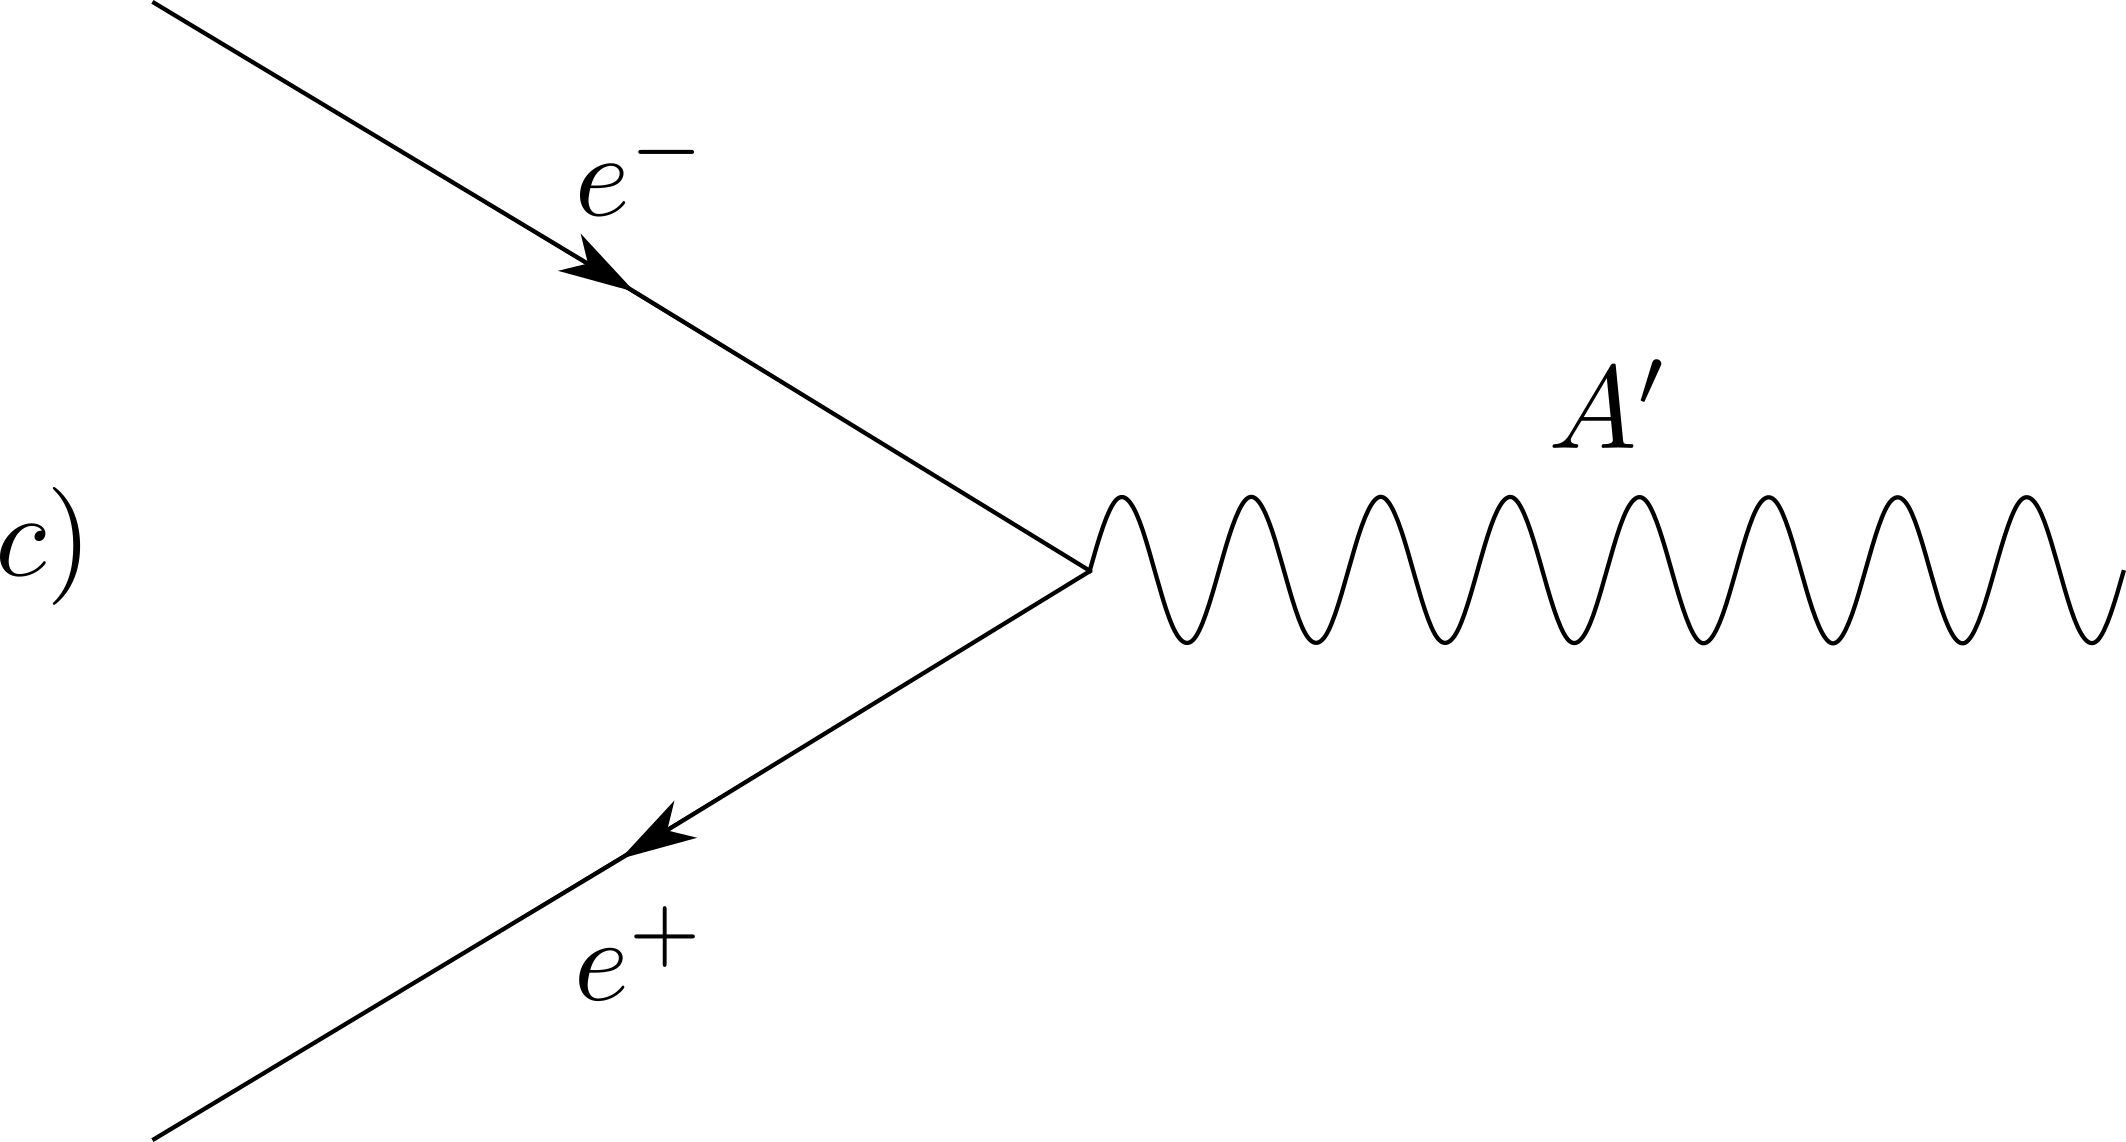
\includegraphics[width=.45\textwidth]{\pdirtwo/DarkResonance.png}
  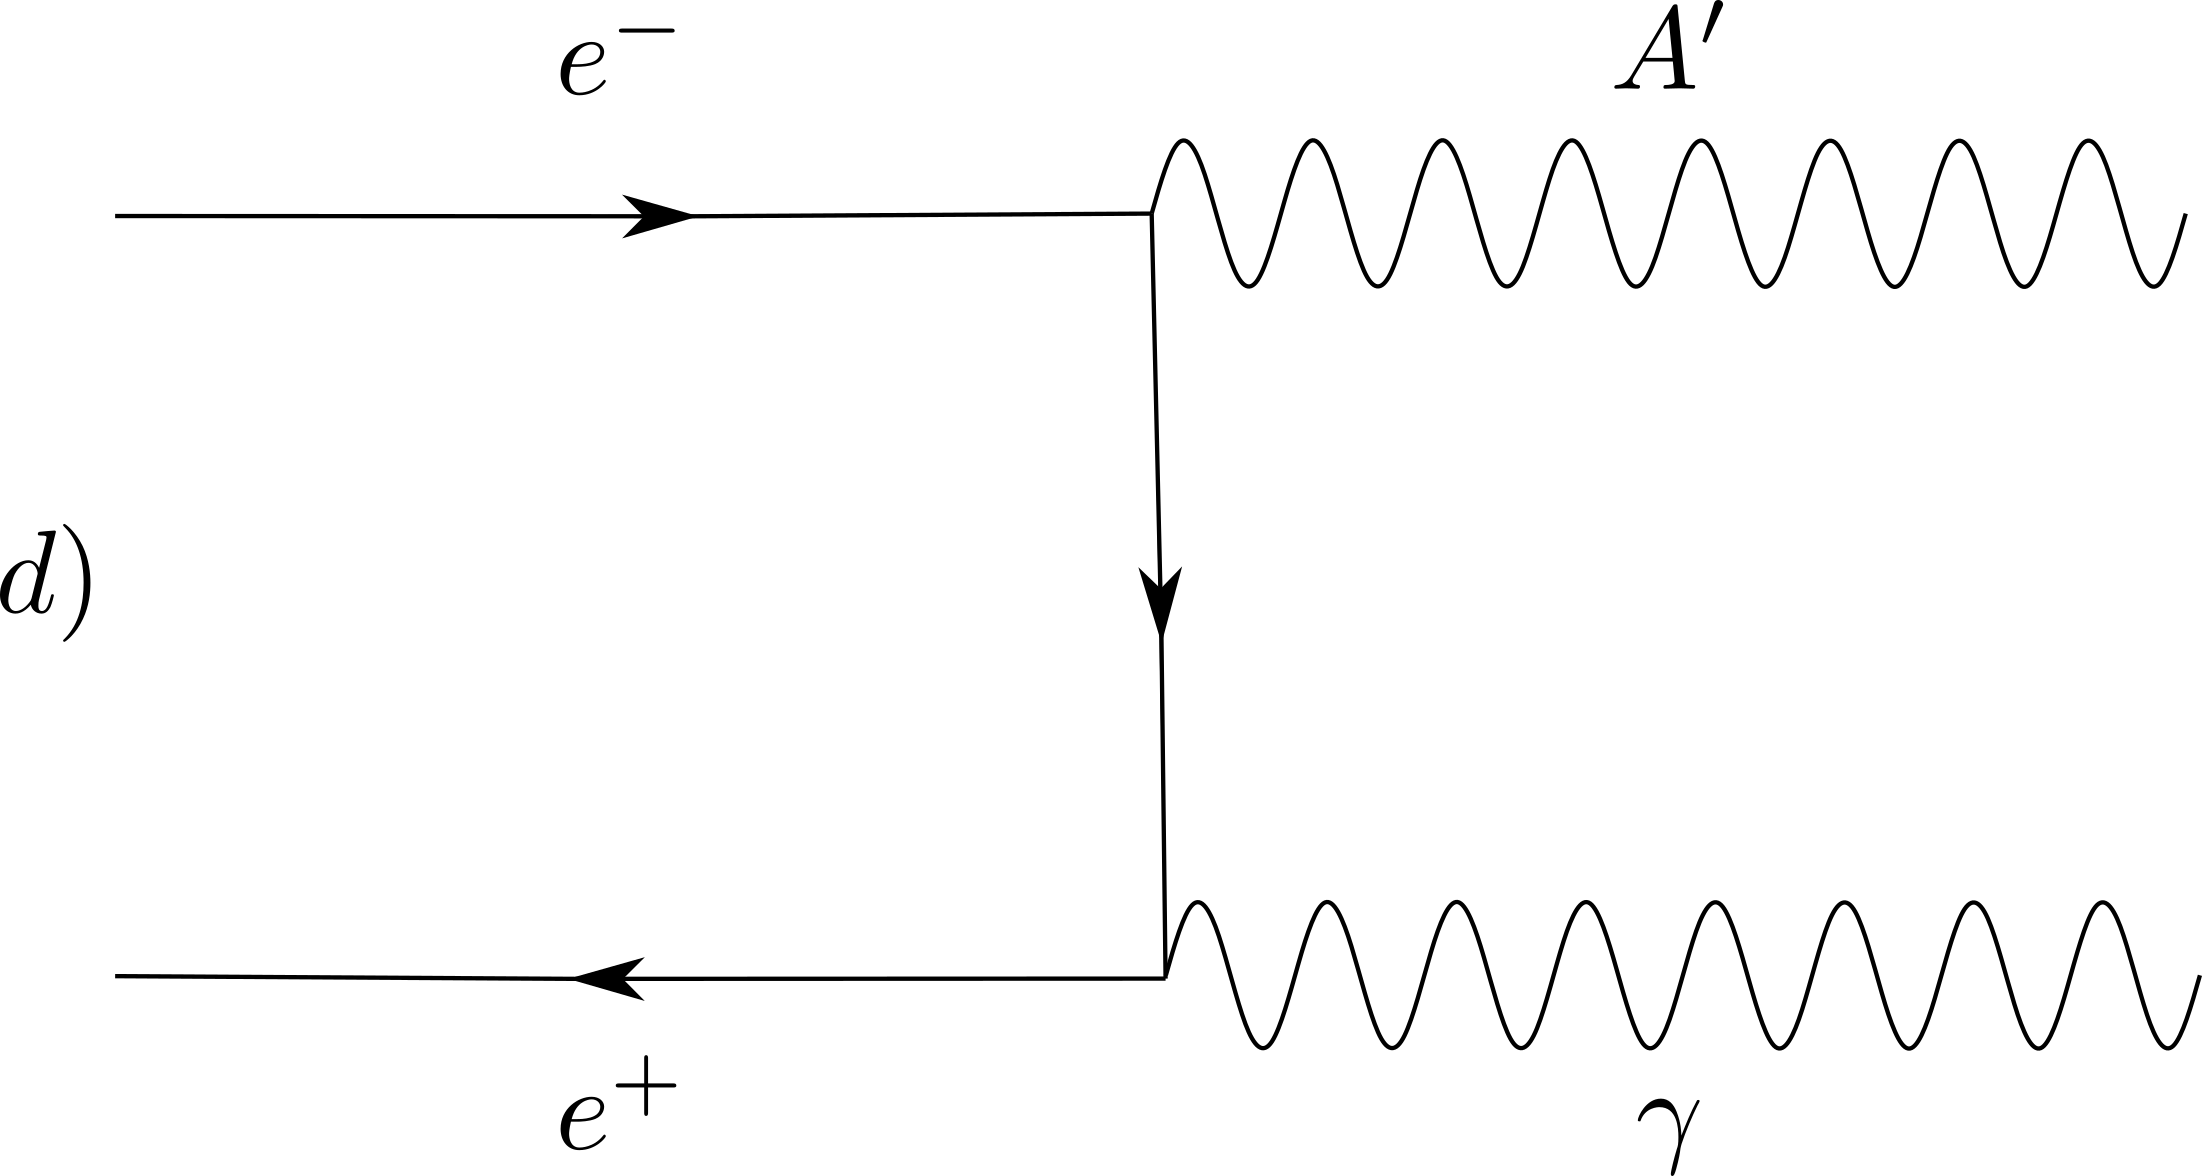
\includegraphics[width=.45\textwidth]{\pdirtwo/DarkAresonance.png}
  \caption{Possible production mechanism for $\DM$: Dark Bremsstrahlung a), Dark Compton b), resonance production c) and A-resonant production d).}
  \label{fig:dm-production-mechanism}
\end{figure}

One has to be careful and consider the list above a simple guideline that is in no way exhaustive. Other channels might be possible with minimal extension of the model, or one could find a significant yield of production not only in the scattering of an electron but also in more exotic physic. An example would be using the electromagnetic portion of large hadron shower to compute the yield of $\DM$. This was for example claimed to be a useful method to search for low mass $\DM$ in \cite{Celentano:2020vtu}.

A careful reader might object that the particles needed for each production channel are different. Indeed while a nuclei Z is always present in matter, the presence of a $\gamma$ or a $e^+$ might not be as straightforward. We remind here however, that in an electromagnetic shower originated by an high energetic lepton all three particles will be produced in large quantity due to the subsequent process of pair-production and Bremsstrahlung that are the most relevant for high energetic $\gamma$ and high energetic $\ee$ respectively. A complete review of electromagnetic and hadronic shower can be found here \cite{Bichsel:2002cf} for the interested. Indeed the production mechanism will be more relevant later when the analysis is performed, in normal circumstances when an high energetic particle hit a thick target all of the mentioned mechanism will be relevant to some degree. In our case, the Dark Bremsstrahlung $\darkbrem$ is used "Golden Channel" for the production. The reason is that it is relatively easy to compute using analytical formulas in good approximation (see Appendix\ref{appendixA:sec:cross-section} for more details) and has a very good yield compared to the other channels. This is not to say that the other channel do not matter, but at this stage where the experiment is being design we will consider them as minor corrections to a production rate mostly dominated by the Dark Bremsstrahlung. To avoid confusion in the reader, we also admit here that an appropriate analysis might make such contribution very relevant. An example can be found in \cite{Marsicano_2018} where the non-resonant and resonant production are used to improve significantly the signal yield for specific mass range.

After the production mechanism is chosen, some first estimate on the signal yield can be performed. However successfully producing the particle is not by itself sufficient without a mechanism device to detect it. The question that becomes interesting here is: what happens to $\DM$ after it is produced inside a target? We remind the reader here that since a coupling between standard matter and dark matter was theorized in the $\umodel$ model, the $\DM$ will be able to decay in a $\ee$ pair (or in more massive leptons) provided that its mass is sufficiently large, but it could also decay in particles of the dark sector, the one called $\dmchi$ introduced in Sec.\ref{chapter1:sec:dm-u1model}. The exact branching ratio can be calculated to be:

\begin{equation}
  \label{chapter1:eq:dm-bratio}
  \Gamma(A'\rightarrow\dmchi) = \frac{\alpha_D}{3}m_{A'}(1 + \frac{2m^2_{\chi}}{M^2_{A'}})\sqrt{1 - \frac{4m^2_{\chi}}{M^2_{A'}}}   
  \Gamma(A'\rightarrow\dmchi) = \frac{\alpha \epsilon^2}{3}m_{A'}(1 + \frac{2m^2_{e}}{M^2_{A'}}\sqrt{1 - \frac{4m^2_{e}}{M^2_{A'}}} 
\end{equation}

To simplify, we consider the two cases where the branching ratio is dominated by one single decay

\begin{itemize}
\item \textbf{Invisible decay:} If $\alpha_D / (\alpha \epsilon^2) \gg 1$ the A' will decay mainly in $\dmchi$. This decay is called invisible, as the decay products interact very weakly with standard matter
\item \textbf{Visible decay:} If $\alpha_D / (\alpha \epsilon^2) \ll 1$ the A' will decay mainly in $\ee$. This decay is called visible, as the decay products can be easily detected since they posses an electromagnetic charge. 
\end{itemize}

As always we need to admit that the physics always offer a plethora of possibilities that are not always easy to summarize in a thesis. There is no meaningful constraint that prevent both branching ratio to be on a similar footing. Likewise models with more complicate decay are possible. An example is the one illustrated in \cite{Mohlabeng_2019}, where the decay chain $\dmsemivis$ dominates. It is of course possible to adjust the setup to be more sensitive to specific model that turn out to be interesting, but in the interest of time we will focus on the two channel explained above that outside of being interesting are the main interest of the NA64 experiment.

The technique used in NA64 to detect this two channels will be explored in Sec.\ref{chapter2:sec:experimental-technique}. After that, the two setup designed for each of the specific two cases will be described in Sec.\ref{chapter2:sec:experimental-setup}. Finally, a detailed description of each detectors involved and their purpose will be outlined in Sec.\ref{chapter2:sec:detectors}.


\section{Experimental Technique}
\label{chapter2:sec:experimental-technique}

The detection of the $\DM$ needs to follow different strategies depending on what decay channel it is favored by it. If $\DM$ decays mainly into $\dmchi$, one could try to detect one of the two particles using a very thick detector. Indeed this is possible since by definition in the $\umodel$ a portal exist that connects dark matter to the classical one. However such an experiment will have a very limited reach, not only a factor $\alpha \epsilon^2$ needs to be "paid" to produced $\DM$ but an additional $\alpha \epsilon^2$ is also needed in order to detect its decay product. It is clear that especially for low coupling $\epsilon$ the probability to detect a single $\DM$ becomes  vanishingly  small. The second possibility is to make the disappearance of energy the signal of the experiment, i.e. assuming that the energy of $\DM$ is completely lost in the event. Such an experiment needs only to produce $\DM$ and does not need to worry about what happen to the particle after. To design a setup able to characterize this type of signature properly, we need to worry about the following items:

\begin{itemize}
\item The initial momentum of the particle needs to be well known
\item The setup needs to be completely hermetic, i.e. no energy can escape detection without using the channel under study
\item The initial particle ID needs to be well known
\end{itemize}

While the two first item are fairly trivial, one could wonder why the last one is necessary. Clearly if we need to apply any kind of statistical analysis to our data one has to know the total number of the electron that impact our target, the so called Electron On Target (EOT), so in this sense to understand the sensitivity of the experiment suck knowledge is necessary. On top of this however, the particle ID is necessary also to distinguish events that are in our signal box even if no $\DM$ is being produced. A precise background discussion is left for Chapter \ref{chapter3}, here we just provide the example of the decay chain $K^- \to e^- \nu_e$ \cite{review-particle-physics}: if a $K^-$ hits the target without being properly distinguished, it is possible for it to leave an electromagnetic signature and at the same time transport some energy out of the setup via $\nu_e$. This is exactly the signature we would expect for $\DM$! Hence the necessity of some system able to distinguish between particle of different species.

What about the visible mode? If we assume the decay $\aee$ is prominent, it is clear that missing energy can no longer be considered a signature. One should search for a $\ee$ pair in the final state, these particles are however very common in particle physics experiment, so one has to think how to characterize the event more. The property that mostly characterize dark matter is its inability to interact with ordinary matter, and hence travel freely inside very dense material. Since $\DM$ travels for a finite distance before decaying, if the target is thick enough, the only way to see an $\ee$ emerging from the target will be that a $\DM$ is being produced. A simple $e^-$ will be stopped by the thick target and nothing will emerge on the other side of the wall. If on the other hand we measure an high-energetic $\ee$ pair emerging on the other side of the wall and the energy of this pair matches exactly the one that is missing from the target, we conclude that the energy was transported outside the volume using a neutral boson. Assuming that no such channel exist in the standard model (which is to be demonstrated with a detailed background study) we can claim the observation of an event compatible with our hypothesis! Noticed in this case as well the three properties listed above are necessary, indeed one needs to know with good precision the initial momentum of the particle hitting the target and be sure that the particle is an electron. In this case however, the signal is not missing energy but instead energy conservation between a detector placed upstream and the one placed downstream. This concept is similar to what is used for Axion searches, the so called "Light Shining Through a Wall" experiments, where the two photons of the Axion decay are detected downstream a very thick wall (for a review, look here \cite{Jaeckel:2010ni}).
If we assume the energy of the primary electron to be $E_0$ and we plot the energy recorded in the two calorimeter, we can conceptualize the difference between the two signature in Fig.\ref{fig:two-signature}. As one can see, we are assuming here that the first calorimeter is able to stop the incoming particle with 100\% efficiency, and that therefore the only way to reach the downstream calorimeter is via the production of dark matter. Although this is mostly the case if the incoming particle is an $e^-$, to probe the $\umodel$ one has to collect a huge number of EOT, in the order of $10^{12}$, it is clear that one a statistic so high is collected even event with a very small chance to happen need to be properly studied. A good setup should not only implement the fundamentals described above but also suppress as much as possible all the background that can potentially leak in the signal box.

\begin{figure}[bth!]
  \centering
  
  \caption[two signature sketch]{Sketch of the two possible signature in a collider setup to probe the $\DM$ existence.}
  \label{fig:two-signature}
\end{figure}

\subsection{invisible decay mode}
\label{chapter2:sec:experimental-technique-invis}

\subsection{visible decay mode}
\label{chapter2:sec:experimental-technique-vis}

\section{Experimental setup}
\label{chapter2:sec:experimental-setup}

In collider experiments, the first choice of a facility to provide the initial beam for the experiment can be crucial. A good initial beam with a low fraction of impurities and good momentum definition can dramatically change the background condition. The NA64 experiment uses the upgraded H4 electron beamline at CERN SPS. The beam is produced by the primary proton beam of 450 \si{\giga\electronvolt} with an intensity up to 10$^{12}$ Proton On Target (POT) per SPS spill. The electrons are produced on a primary beryllium target and transported to the detector inside the evacuated beam-line tuned to an adjustable beam momentum. A precise description of the beam apparatus can be found here \cite{sps-beamline,h4-beamline}. The beam properties can be tuned for the precise experiment, hence its precise property can depend on the target used for the conversion, the magnetic field employed and other components. In the case of NA64, two different composition are used depending on which $\DM$ decay is being probed. In the case of the invisible decay $\ainv$, the beam momentum is tuned to 100 \si{\giga\electronvolt}. In this condition, a purity $\pi^-/e^- \lesssim 10^{-2}$ is achieved with a beam size of $\sim$1.5\si{cm} (FWHM). In the case of the visible decay $\aee$ on the other hand, a large initial energy can be helpful to boost the decay time of the $\DM$ outside the target and therefore increase the sensitivity of the setup. This is especially true for the $\DMX$, since an important portion of the parameter space justifying this anomaly is characterized by large coupling $\epsilon \gtrsim 10^{-3}$ and hence a decay time $\tau \lesssim 10^{-13}$\si{s}. In this case, the beam is tuned to 150 \si{\giga\electronvolt} as a compromise between high-energy and small beam degradation.

In the next sections both of the setup used by NA64 will be described in detail. Since the physics happening is the same before the electron hits the target, the two setup shares many similarities. We will follow here an historical approach where we will described first the invisible mode setup which was first used in the test beam of 2016. In Sec.\ref{chapter2:sec:vismode} on the other hand we will focus on the most important difference between the two setup.

\subsection{The invisible mode setup}
\label{chapter2:sec:invismode}

The NA64 invisible mode setup has changed slightly during the year as the understanding of the specific problems in the $\DM$ search were discovered. In the interest of time, we will here described 

After the 100 \gev e$^-$ enter the setup, its momentum needs to be measured precisely to provide an initial estimate of its energy. This is achieved using a magnetic spectrometer using an integrated field of $\sim 7 T \dot m$ achieved using two dipole magnets \cite{mbpl} placed in series along the primary axis of the beam. The entrance angle of the particle inside the magnet is defined by two Micromegas (MM) trackers placed inside the 5 m space between the beam inlet and the first magnet entrance. Between the two MM, in a space of approximately 2 m, two scintillators ($S_{0-1}$) and a V counter are placed to ensure a proper beam definition. The V counter consist in a scintillator with a hole in the middle, and is used to reject particle with a high beam divergency that could in principle be a source of background. After the two magnets, a vacuum tube kept at the pressure of approximately 10$^{-3}$ \si{mbar} is placed immediately after for a total length of 10.2 \si{m}. The vacuum tube minimize the interaction of the particles during its travel to the target, this is clearly important to reduce the energy lost of the primary e$^-$ before its energy is measured again in the ECAL, but as will be detailed in Sec.\ref{chapter3:sec:bkg-srd} reducing the ionization increases the background suppression achievable with synchrotron radiation. After the vacuum tube, an additional space of $\sim$ 4.5 \si{m} contains the last detector before the target. A second set of three scintillators ($S_{2-3-4}$) complete the triggers. Three set of Pb-Sc sandwich are placed in the arch contained between the original beam and the bent beam direction to collect the synchrotron radiation emitted in the magnetic field upstream. On the other side of the beam, another similar detector with no transversal segmentation (W sandwich) is placed to reject events with high beam divergency or where the electron experienced an high energy scattering upstream. Four more MM are placed along the beam to complete the momentum reconstruction by detection the precise hit position of the electron after its passage through the magnetic field. Eight more tracking detectors are placed before the ECAL: 2 Strawtubes (St), 2 Hodoscope (H) and 4 four Gas Electron Multiplier (GEM). The GEM detectors have a similar hit resolution and efficiency similar to the MM, with the advantage of not being multiplexed, hence they experience less redundancy in the hit position at the cost of a larger number of channels. As it will be detailed in Sec.\ref{chapter2:sec:detectors-tracking} the multiplexing does not limit the momentum resolution and hence the final performance given are comparable overall. The strawtubes and Hodoscope on the other hand posses a larger active area ($\sim$0.5 m), but an hit resolution of $\sim$1\% which makes them less suitable to reconstruct the momentum precisely (insert here straw reference?). This detector have however the virtue of being large enough to detect charged particle emitted at a large angle, and hence can reject some rare events that are produced by an inelastic scattering of the incoming particles on one of the MM modules placed downstream. This events although rare, cannot be catched by the W and they can be a source of background for the large number of EOT required by the experiment \cite{na64-prd}. 

After this region is passed, the primary electron finally hit the active target (ECAL). Here the energy of the electron is measured again by stopping the particle completely. The ECAL is made of 36 modules arranged in a 6$\times$6 matrix, each modules has a Pb-Sc structure with 150 layer for a total of 40$X_0$. Due to its transverse segmentation, the ECAL allows further background rejection using a shower profile analysis to distinguish between an em-shower and an hadronic one. To ensure complete hermeticity, an high efficiency VETO and a large Hadronic CALorimeter (HCAL) are placed after the ECAL target. The VETO consist in three separate scintillator stacked together for a total thickness of 5\si{cm} and reject MIP with an estimated efficiency of 99.9$\pm$0.1\%. The HCAL placed immediately after consist of four modules of $\simeq$7 $\lambda_{int}$ (nuclear interaction length) each. Each module is built in a 3$\times$x matrix of single Fe-Sc sandwich array. The role of this last calorimeter is to block all possible particle penetrating the ECAL and grants complete energy hermeticity to the setup. In the past version of the setup, all four modules were stacked in series after the ECAL to grant a total of $\simeq$28 $\lambda_{int}$. In the more recent version of the setup from Fig.\ref{fig:setup-invis-2018} however, the last module is shifted to face the original beam axis. After the first test beam it was clear that the additional background suppression of a fourth module was not needed. Instead the last module is used to gain insight to the neutrals in the beam and can catch large bremstrahlung photons emitted before the magnet by the incoming electrons. A more detailed description of all this detector can be found in \ref{chapter2:sec:detectors}.


\begin{figure}[tbh!]
  \centering
  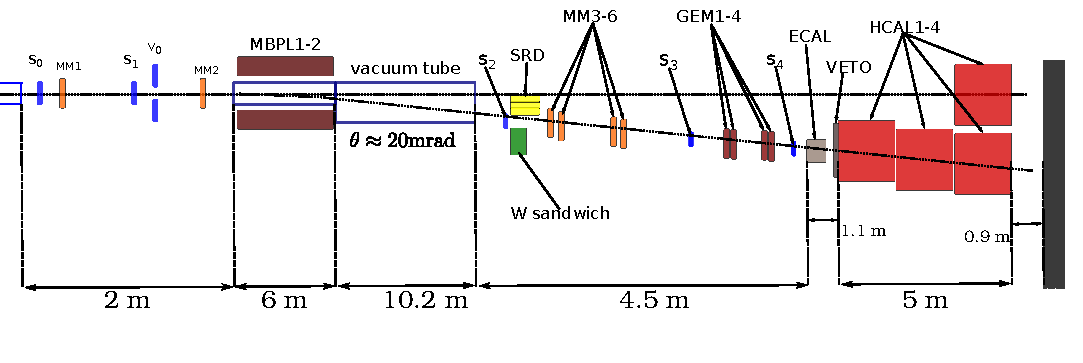
\includegraphics[scale=0.8]{\pdirtwo/setup-invis-2018.pdf}
  \caption[invisible mode setup 2018]{Invisible mode setup 2018, top view.}
  \label{fig:setup-invis-2018}
\end{figure}

\subsection{The visible mode setup}
\label{chapter2:sec:vismode}

The visible mode setup is obtained by modifying slightly the invisible mode setup to accomodate the $\aee$ decay in a long decay volume where the $\ee$ pair is measured by a scintillator counter and four GEM station (Fig.\ref{fig:setup-vis-2018}). The energy of the beam is increased to 150 GeV. The reason for this is to boost the decay time of the $\DMX$ in order to increase its probability to leave the dump. As a consequence, the total displacement in the X-direction of the primary beam is roughly $\sim$10 \si{mm} smaller. Since the space between the origin and bent beam axis is reduced, only two module of the SRD detector can be placed in this space, which decreases the suppression of heavy charged particles. Additionally, the smaller bending have an impact on the momentum reconstruction as well, this however is not very significant for this analysis. Since no energy evaporates in this mode, there is no direct need to compare two different energy measurement. Instead, another compact calorimeter made of a Tungsten-scintillator sandwich (WCAL) is placed in front of the ECAL and act as the target in this new setup. This calorimeter has a total of 30$X_0$ in a compact length of $\sim$20 \si{cm}. The $\DM$ is produced via scattering off nuclei in this active dump, followed by its decay $\aee$ after traveling for some distance without interaction. To ensure that the decay happens after the dump, the last two layers of the WCAL read separately (W2), and act as a VETO to stop high energetic particle that leak from the em-shower to enter the decay volume undetected. A vacuum tube of 3.1 \si{m} kept at a pressure of $\sim$10$^{-2}$ \si{mbar} is placed immediately after the dump to minimize interaction of the $\ee$ after the decay. A scintillator (S$_4$), is placed immediately after the tube to detect the presence of the $\ee$ pair with double-MIP signal inside this counter. A set of four GEM detectors are then placed in the last $\simeq$2.5 \si{m} of air before the second active target (ECAL). In principle this four trackers can reconstruct the angle and the vertex of the decay to offer an additional characterization of the signal. These tools were not used in the analysis performed in 2018 \cite{Banerjee:2019hmi}, but in this work an analysis considering the trackers as well is described in detail (see Sec.\ref{chapter3:sec:vis-mode-tracking}). Finally, the ECAL detect the remaining energy of the two $\ee$ pair in the decay volume, and matches it to the one measured in the WCAL. If the sum $E_{WCAL}+E_{ECAL}$ is compatible with the initial primary energy E$_0$, we conclude that some energy escaped the first dump WCAL using a channel not compatible with the standard model of particles. At the tail of the setup, an high-efficiency VETO and the HCAL are still presented to guarantee again the hermeticity of the setup similarly to the invisible mode. One could question the usefulness of these detectors in this mode. Indeed if we can guarantee that only 150 GeV $e^-$ are in the system, the simple requirement of energy conservation should be enough to reject all backgrounds coming from impurities in the beam. Again here we need to remember that the many assumption made in theory can encounter many problem in practice. The pileup of two different events, one hadronic and one electromagnetic, could easily break this assumption. The limited energy resolution of the two calorimeter can likewise produce in rare occasion a wrong measurement that implies energy conservation in an event. On the top of this, the HCAL is invaluable to properly estimate the hadron contamination of the beam (and therefore the precise number of EOTs accumulated) and to select the rare event $\emu$ where two muon are produced in the dump inside the em-shower. As we will see this type of event is crucial for our analysis to properly account for the systematic of the experiment, both in the invisible and visible mode, which makes the HCAL and VETO necessary for both setups.

\iffalse
The method of the search for $\aee$ (or $\xdecay$) decays is detailed in . Here, we review it briefly. The $\DM$ is produced via scattering of 150 GeV electrons off nuclei of an active target-dump. The $\DM$ production is followed by its decay into $\ee$ pairs:
detailed in \cite{Gninenko:2013rka, Andreas:2013lya, gkkk1, DMsimulation}, 
\begin{equation}
e^- + Z \to e^- + Z + \DM   ;~ \DM\to \ee \,.
\label{ea}
\end{equation}
\fi

\begin{figure}[tb]
\centering
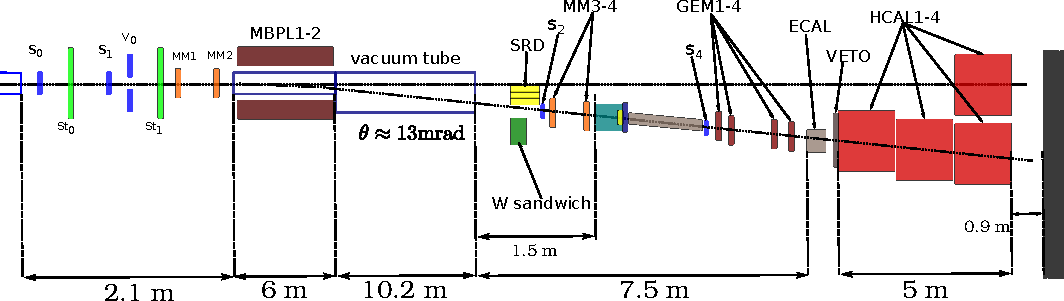
\includegraphics[width=1.\textwidth]{\pdirtwo/NA64_setup_2018_visible.pdf}
\caption[NA64 visible mode setup 2018]{The setup to search for $\DM$$\to \ee$  decays of the bremsstrahlung $\DM$ produced in the reaction
$eZ \to eZ+\DM $ of the 150 GeV electrons incident on the active WCAL target.}
\label{fig:setup-vis-2018}
\end{figure}

\section{Detectors}
\label{chapter2:sec:detectors}

In this sections the various detectors that are used to build the two setup described above are described in more detail to give a technical overview of each component of the setup. More information about each detectors are detailed in \cite{na64-hcal,na64-detectors,ABBON201569}. 

\subsection{The Trigger system}
\label{chapter2:sec:detectors-trigger}

The trigger system is based on the coincidence and anti-coincidence of different scintillator counters placed along the beam directions and the requirement of a specific energy in the primary active dump (the ECAL in the invisible mode and the WCAL in the visible mode).

Five plastic scintillators (S$_{0-4}$) and one Veto (V) are used in the NA64. They have a variable diameter ranging from 32 to 42 \si{mm} and a thickness of 3-5 \si{mm}. The sandwich S$_0$-V-S$_1$ is placed in front of the beam inlet to characterize the initial particle direction. To pass this first step of the trigger, a particle need to leave a signal of $\sim$0.8 MIP in S$_{0-1}$ and no signal in V, i.e. following the condition:

\begin{equation}
  \label{eq:trigger-upstream}
  Tr_U = S_0 \cdot \bar{V} \cdot S_1
\end{equation}

The signal need to be in a coincidence compatible with the time resolution of the two scintillators ($\simeq$3 \si{ns}) to suppress the pileup. Downstream, three more scintillator are placed (S$_{2-4}$) in the case of the invisible mode (See Fig.\ref{fig:setup-invis-2018}) and a coincidence of all three is also required as a part of the trigger downstream. In the case of the invisible mode, only the first of three scintillator (S$_2$) is part of the trigger, S$_3$ is removed and S$_4$ is placed after the decay for analysis purpose without being a direct part of trigger. This means:

\begin{equation}
  \label{eq:trigger-downstream}
  Tr^{invis}_D = S_2 \cdot S_3 \cdot S_4
  Tr^{vis}_D = S_2
  Tr_{U+D} = Tr_U \cdot Tr^{invis/vis}_D
\end{equation}

In this case, we notice that the scintillator S$_2$ downstream is small enough to already limit significantly the range of momenta accepted in the trigger of the experiment ($\gtrapprox$ 90 \si{\gev})). However large beam divergency coupled to trigger pileup can still potentially accepted a low energy $e^-$ inside the setup, hence the necessity of a tracking system. As final tool for the beam definition, a small energy deposit in W is required, to reject event with a large upstream bremsstrahlung. The exact threshold is not consistent between different runs, but it is always in the range of 3-6 \si{\gev}. We define the beam-trigger as the sum of all these components in the two different setups:

\begin{equation}
  \label{eq:trigger-beam}
  Tr_{beam} = Tr_{U+D} \cdot \bar{W}
\end{equation}

Finally, as the DAQ can collect data at a rate of $\simeq$10 \si{kHz}, one need an additional condition to select only those events that have a chance to be in the signal region. In both setup, this means some missing energy in the primary target-dump. Additionally, since both WCAL and ECAL have some longitudinal segmentation, one can use the pre-shower information to suppress the hadron background at trigger level. This is achieved by splitting the signal in these modules to feed them to a discriminator. The trigger in this case has the following form:

\begin{equation}
  \label{eq:trigger-phys}
  Tr^{invis}_{phys} = ECAL^{presh}(>300 MeV) \cdot ECAL(<85 GeV)
  Tr^{vis}_{phys} = WCAL^{presh}(>500 MeV) \cdot WCAL(<110 GeV)
\end{equation}

The final trigger during data taking will be a combination of both the primary trigger for the beam definition and the physical trigger used to obtained a rate that can be handled by the DAQ. We obtain finally:

\begin{equation}
  \label{eq:trigger-total}
  Tr^{invis}_{total} = S_0 \cdot \bar{V} \cdot S_1 \cdot S_2 \cdot S_3 \cdot S_4 \cdot \bar{W} \cdot ECAL^{presh}(>300 MeV) \cdot ECAL(<85 GeV)
  Tr^{vis}_{total} = S_0 \cdot \bar{V} \cdot S_1 \cdot S_2\cdot \bar{W} \cdot WCAL^{presh}(>500 MeV) \cdot WCAL(<110 GeV)
\end{equation}

The precise definition of the trigger varies between different runs. In general we can define three different runs:

\begin{itemize}
\item \textbf{Hadron calibration run:} Where $\pi^-$ is used as primary particle and only $Tr_{beam}$ is used. This runs are used to measure precisely the interaction of such heavy charged particle in the setup to study precisely the background suppression in NA64. Their intensity is suppressed due to the thick target placed inside the beamline ($\lesssim 10^{-3}$ $\pi^-$\si{\per\second}).
\item \textbf{Electron calibration run:} Where $e^-$ is used as primary particle and only $Tr_{beam}$ is used. This runs are used to measure the typical interaction of an EOT without the a physical trigger that biases the final distribution. 
\item \textbf{Physical run:} Where $e^-$ is used as primary particle and both $Tr_{beam}$ and $\Tr_{phys}$ are used. This runs contain all the data used for the final analysis. 
\end{itemize}

We remind here that although the Physical runs use an electron beam, the physical trigger used naturally selects events with hadrons as a primary particle. This is obvious from the fact that the vast majority of $e^-$ will deposit all their energy inside the target-dump, hence will be reject by the physical trigger. This means that the sample of events recorded will have a large percentage of hadrons that will be rejected by the selection criteria. To properly account for the cuts efficiency, electron and hadron calibration runs are used , since the impurity of the sample is well known and easy to remove. The most classical approach to remove the impurity is an SRD cut: electrons can be selected or rejected by measuring the presence or absence  of the synchrotron radiation in the SRD crystals. This improve the purity from a $\lessim 1\%$ to $\lessim 10^{3}\%$ therefore permitting precise studies on the various cuts. 

\subsection{The Electromagnetic Calorimeter (ECAL)}
\label{chapter2:sec:detectors-ecal}

The electromagnetic calorimeter shown in Fig.\ref{fig:ecal-sketch} is a shashlik type detector design for energy measurement, shower profile measurement and $e/\pi$ separation. Its design consist in a 6$\times$6 matrix of single modules with dimension 38.2$\times$38.2$\times$471 \mmc. Each cell consist of 150 layers, which in turn are made of 1.5 \mm as converter layer, 0.14 \mm of paper as separator and 1.5 \mm for energy measurement. This is equivalent to 40$X_0$ radiation length. The single cell is further divided in two different longitudinal segment. The first one is called pre-shower and consist of 16 layer ($\sim$4.27$X_0$) and gives resolution to the very beginning of the shower. Since $e^-$ and $\gamma$ trigger an em-shower very early (with the $\gamma$ being a bit delayed within respect to the electron. see \cite{Bichsel:2002cf}), this information can be used to discriminate such particles from all the ones with higher penetrating power (mostly $\pi^-$ and $\mu^-$ in the NA64 case). The second part called simply main ECAL consist in the remainder of the 134 layers ($\sim$35.73$X_0$), and its purpose is to complete stop the incoming particle to measure its energy. The light collection of the scintillator part is performed by WLS fibers BCF91a \cite{wls-fibers} inserted in spiral along the cell in order to avoid energy leak through them. The Calorimeter is calibrated using a low intensity electron beam where a mechanical support structure is used to move each single cell on the beam center. The pre-shower and the main calorimeter are then calibrated using a Gaussian fit and the precise energy fraction between the two longitudinal segment is calculated through a detailed MC simulation. The energy resolution estimated for this detector is of $10\% / \sqrt{E[GeV]}$.

\begin{figure}[bth!]
  \centering
  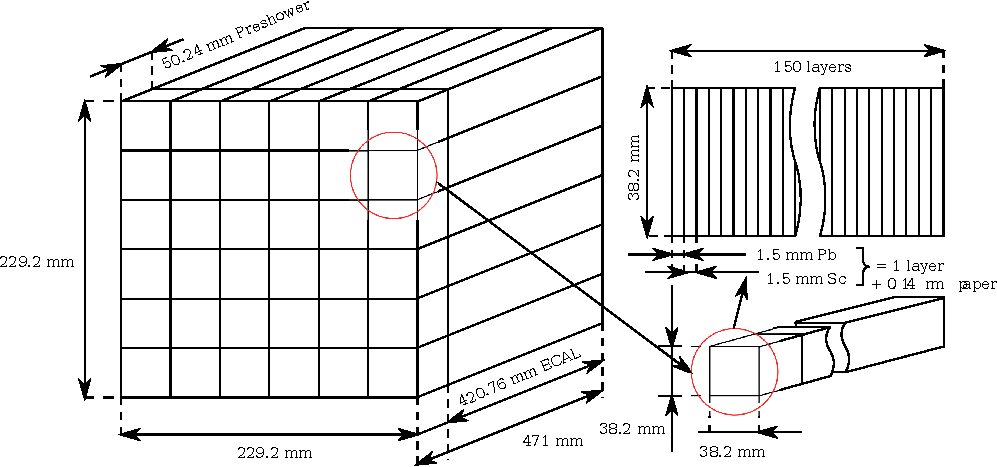
\includegraphics[scale=1]{\pdirtwo/ECAL.pdf}
  \caption[ECAL sketch]{Technical sketch of the Shaslik type calorimeter.}
  \label{fig:ecal-sketch}
\end{figure}

\subsection{The Hadronic Calorimeter (HCAL)}
\label{chapter2:sec:detectors-hcal}

The hadronic calorimeter in the NA64 experiment consist in four modules and its primary purpose is to stop and reconstruct the energy of high penetrating particle. This includes the $\pi^-$ and $K^-$ contained as impurities in the beam but also neutrons and protons that can be produced in inelastic scattering in the ECAL. Additionally, although a complete stop of 100 GeV $\mu^-$ remains unfeasible, the HCAL can characterize very efficiently the presence of such particle after the ECAL, as the $\mu^-$ will leave the very distinctive MIP energy deposit inside each module, amounting roughly to $\sim 2.5$ \gev. Each module of the HCAL is a 3$\times$3 matrix of cells. Each cell is a sandwich of alternating layers of 25 \mm Iron (Fe) and 4 \mm of scintillating material separated by a 9 \mm gap  of air. Each cell consist of 48 such layers for a total thickness of $\simeq 7\lamba_{int}$. The lateral size of each modules is 194$\times$192 \mms. The light readout is analogous to the one of the ECAL, using WLS-fibers embedded in round grooves in the scintillator plates. The fibers from each cell are collected together in a single optical connector at the side of the module. Each of the 9 optical connector is then read-out by a single photomultiplier. Similar to the ECAL, these modules are calibrated using special runs where 50 \gev $\pi^-$ are shoot at different cells with the help of a mechanical table. The energy resolution estimated for this detector is $\sim 50\%/\sqrt{E[GeV]}$

\begin{figure}[bth!]
  \centering
  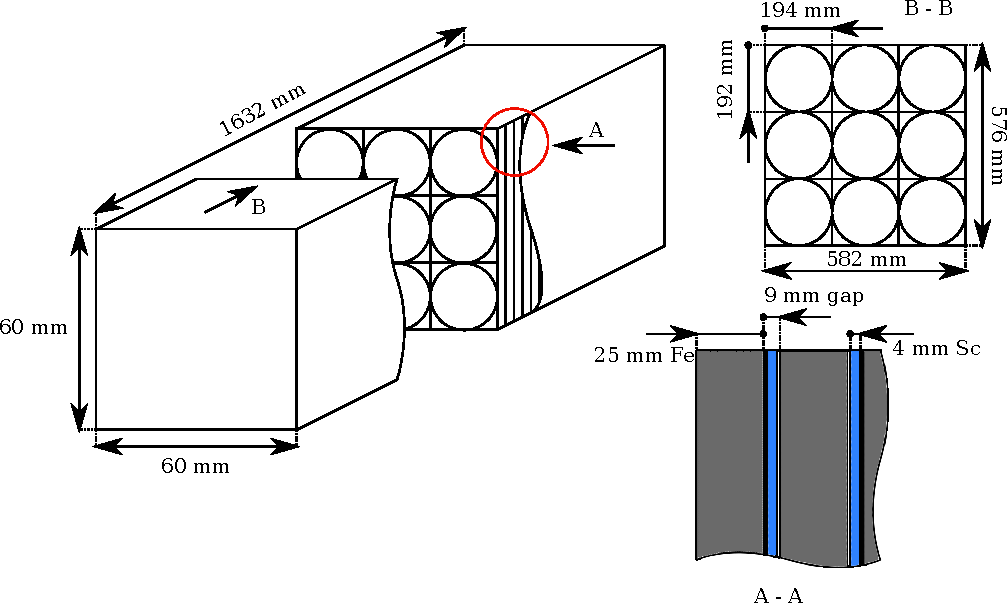
\includegraphics[scale=1]{\pdirtwo/HCAL.pdf}
  \caption[HCAL sketch]{Technical sketch of the HCAL module used in the NA64 experiment.}
  \label{fig:hcal-sketch}
\end{figure}

\subsection{The Synchrotron radiation detector (SRD)}
\label{chapter2:sec:detectors-srd}

The Synchrotron radiation detector (SRD) is a small calorimeter placed downstream in the arc described by the original beam axis and the bent beam. Its purpose is to measure the energy of the photon emitted by the passage of each electron in the magnetic field downstream. The energy range of such signal is in the order of a few tens of MeV, hence the need of a larger precision compared to the calorimeter used to measure the primary beam. The detail of heavy charged particle suppression will be described more in detail in Sec.\ref{chapter3:sec:bkg-srd}, here we described the detector technically.

Historically, the first Synchrotron radiation detector used was a set of 8 BGO crystals arranged in a 2$\times$4 matrix placed parallel to the beam direction. Each crystal has a hexagonal shape with a diameter of 61 \mm and a length of 200 \mm. The light readout consist in a EMI PMT 9603 mount on the bottom of each crystal with optical grease. The BGO are excellent candidate for the SRD, due to the high light-yield and radiation length which coupled to their high Z makes them excellent gamma-absorbers \cite{bgo-crystal}. Indeed their rejection power can be as large as $10^{-4}$ and was demonstrated experimentally thanks in the NA64 experiment (see Sec.\ref{chapter3:sec:bkg-srd} for details). However, their large decay time of $\sim$300 \si{ns} creates a level of pileup that limit significantly their usefulness in a context where the intensity of the beam is very high.

The BGO detector was substituted with a shashlik type detector since the 2017 beam time. It is a shashlik type detector that uses three adjacent cells of dimension 60$\times$80 \mm. Each cell consist in 100 layers with a lead-scintillator structure with dimensions 0.1 \mm and 1.1 \mm respectively. The light is read out by a R9420-100-10 Hamamatsu PMT with extended green spectral sensitivity \cite{hamamatsu-R9420-100-10}.

The time resolution for the shashlik type SRD is of $\sim$5 \si{ns}, which grants a suppressed pileup even at the largest intensity allowed in the H4 beamline.

\begin{figure}[bth!]
  \centering
  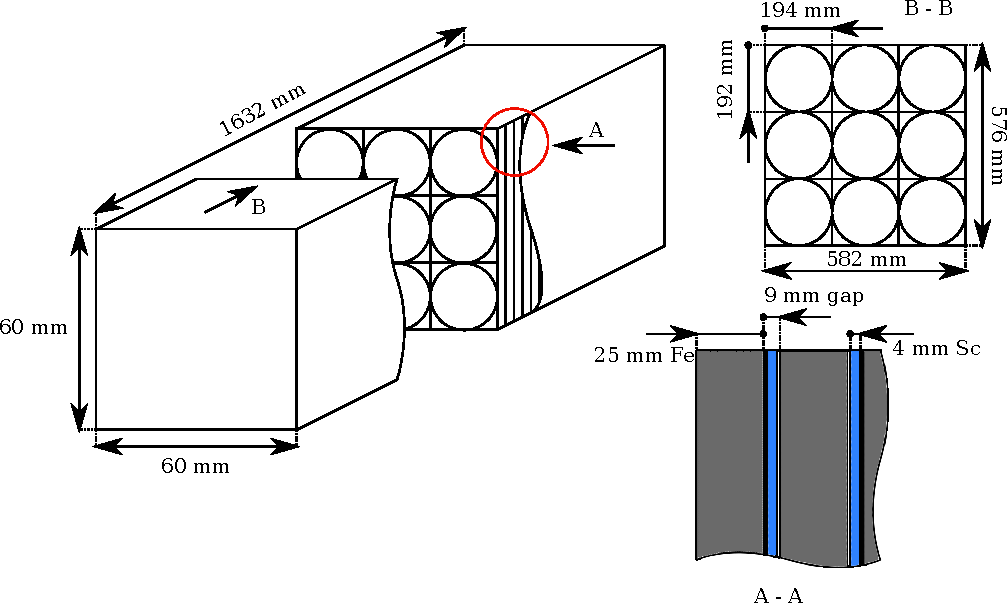
\includegraphics[scale=1]{\pdirtwo/HCAL.pdf}
  \caption[BGO sketch]{Technical sketch of a single BGO crystal.}
  \label{fig:bgo-sketch}
\end{figure}

\begin{figure}[bth!]
  \centering
  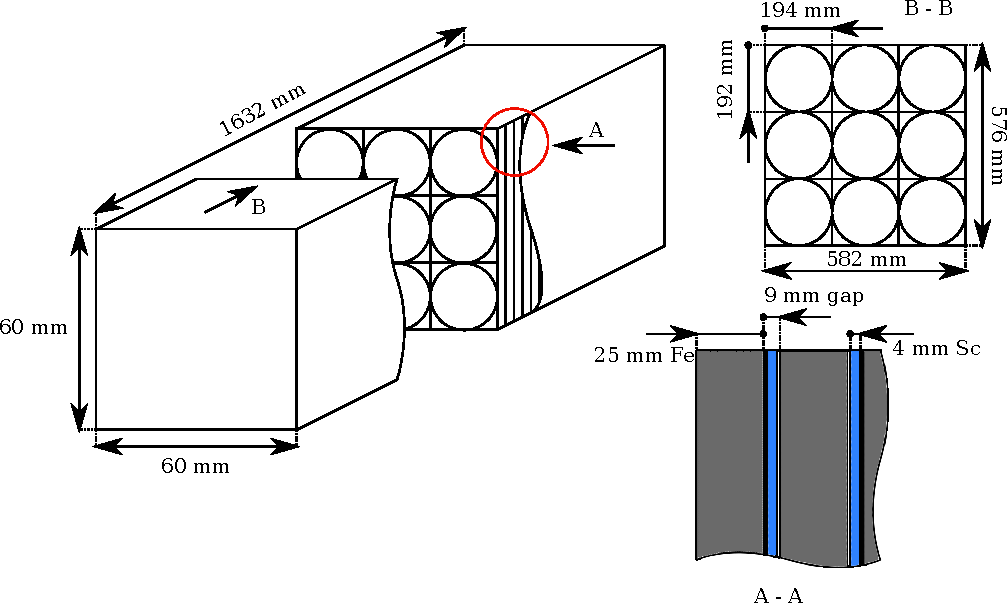
\includegraphics[scale=1]{\pdirtwo/HCAL.pdf}
  \caption[SRD sketch]{Technical sketch of a single shashlik type module used in the NA64 experiment as SRD.}
  \label{fig:srd-sketch}
\end{figure}

\subsection{The Veto system}
\label{chapter2:sec:detectors-veto}

The Veto system is the set of detectors that has the purpose of measuring any particle penetrating one of the NA64 calorimeter to catch event with long longitudinal shower profile that pose a risk to the hermeticity of the setup.

In general, the veto are scintillator counter of variable dimensions that are placed at the end of one of the calorimeter. The most relevant detector of this type is the VETO, a set of three scintillators mounted in series for a total dimension of 550$\times$550$\times$50 \mmc. The MIP inefficiency of this detector is $\sim 10^{-3}$.

For the visible mode, it is crucial to maintain the dump as short as possible to increase the probability of the $\aee$ decay to be outside of the dump. For this purpose the last layers of the WCAL sandwich are decoupled from the main readout and used as veto (called W2). The dimension of this counter are hence connected to the one of the WCAL : 23$\times$23$\times$6 \mmc. For testing purpose, a second thicker counter (called V2) is still placed at a distance of $\sim3$ \si{cm} from W2 to cross check its inefficiency. Such number is then used to compute correctly the signal yield of each run.

In general, a signal event in both visible and invisible mode need is characterized by the absence of energy in the veto counter placed behind that target dump. This is practice typically translates to an energy deposit $<$0.8 MIP to take into account both pedestal and energy resolution of these detectors.

\subsection{The Tracking system}
\label{chapter2:sec:detectors-tracking}

The tracking system is the set of detectors that allows the full momentum reconstruction and track propagation in the NA64 setup. In the NA64 setup four type of detector are capable to reconstruct hits position: Micromegas (MM), Gas Electron Multipler (GEM), Hodoscopes (H$_i$) and Strawtubes (St$_i$). While all of this detector were useful for many different studies performed to analyze the beam composition and estimate the background, to this date only MM trackers are used as direct part of the tracking system. This is to improve the overall efficiency of the selection criteria used for the momentum reconstruction and to limit the systematic of the experiment. In this thesis however, a new analysis of the visible mode data is proposed that uses data from the GEM trackers to reconstruct the vertex position and the angles of the particles in the decay volume. This analysis is detailed in Sec.\ref{chapter3:sec:vis-mode-tracking}.

The exact working principle of each of this detector is beyond the scope of this thesis. This section will be dedicated mostly on the description of the Micromegas detector, that were direct part of every analysis currently performed and furthermore one of my main responsibilities during the whole thesis. For the interested reader, I recommend the thesis of Peter Degen \cite{pdegen-thesis} which I had the pleasure to supervise. In his work he gives a very good overview of the working principle of the straw chamber and compare our modules to the MC prediction in the NA64 experiment.

\subsubsection{Micromegas}

Micromegas trackers are a set of eight Multiplexed XY Resistive Micromegas detectors (MM1-MM8) used to reconstruct the 2D hit position of the incoming particles in the NA64 experiment. The design and original testing of the first modules were already the topic of a previous thesis authored by Dipanwita Banerjee. For a complete review of this detector, I suggested the reader her very good thesis \cite{dbanerjee-thesis} and her article published on this topic \cite{Banerjee:2017mdu}. As shown in Fig.\ref{fig:mm-sketch}, 

\begin{figure}[bth!]
  \centering
  
  \caption[Micromegas sketch]{Sketch of the micromegas detector used in the NA64 experiment}
  \label{fig:mm-sketch}
\end{figure}

\subsection{The data Acquisition system (DAQ)}
\label{chapter2:sec:daq}

%%% Local Variables:
%%% mode: latex
%%% TeX-master: t
%%% End:
